\begin{tabular}{ c c c c }
\adjustbox{valign=m}{%
\begin{lstlisting}[language=C++, basicstyle=\ttfamily\small]
if (x > 0) y = 10;
else y = 20;
\end{lstlisting}
}
&
\adjustbox{valign=m}{%
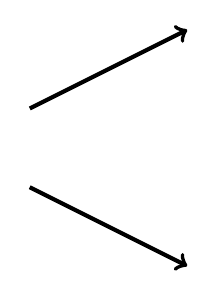
\begin{tikzpicture}
    \draw[->, line width=1.5pt] (0,0.5) -- (2, 1.5);
    \draw[->, line width=1.5pt] (0,-0.5) -- (2, -1.5);
\end{tikzpicture}
}
&
\adjustbox{valign=m}{%
\begin{minipage}{0.4\textwidth}
\textbf{Without Predication:}
\begin{lstlisting}[basicstyle=\ttfamily\small]
    cmp r0, #0
    bgt greater
    mov r1, #20
    b end
greater:
    mov r1, #10
end:
\end{lstlisting}

\vspace{0.8cm} % Space between the two assembly listings

\textbf{With Predication:}
\begin{lstlisting}[basicstyle=\ttfamily\small]
    cmp r0, #0
    movgt r1, #10
    movle r1, #20
\end{lstlisting}
\end{minipage}
}
\end{tabular}